% Choptuik's echo period at large dimension.  Build: see paper/Makefile (pdflatex twice).
\documentclass[aps,prd,onecolumn,superscriptaddress,nofootinbib,11pt]{revtex4-2}
\usepackage{amsmath,amssymb}
\usepackage{graphicx}
\usepackage{booktabs}
\usepackage{dcolumn}
\usepackage[colorlinks=true,linkcolor=blue,citecolor=blue,urlcolor=blue]{hyperref}

\newcommand{\Dinf}{\Delta_\infty}
\newcommand{\eps}{\varepsilon}
\newtheorem{proposition}{Proposition}

\begin{document}

\title{Choptuik's echo period at large dimension: evidence for a finite limit
$\Delta_\infty = 1.64389375$, and selection beyond all orders in $1/D$}

\author{Nathan Moinvaziri}
\email{nathan@nathanm.com}
\noaffiliation
\thanks{Independent. How this work was done is described in Sec.~\ref{sec:how}: the
computations, derivations and text were produced by an AI model (Claude, Anthropic) working under the author's
direction; the author has not checked the mathematics himself, and no human expert has reviewed it.}

\date{October 2026; unreviewed draft}

\begin{abstract}
We compute the echo period $\Delta(D)$ of Choptuik's discretely self-similar critical solution of massless scalar
collapse in $D$ spacetime dimensions at 857 points $8.25 \le D \le 61.03$ with a double-double (about 32-digit)
solver, consistent with smooth curves to $4\times10^{-15}$, and with an independent double-precision solver for
$4 \le D \le 40$. One rational function of $1/(D-2)$ reproduces $\Delta$ and the critical exponent $\gamma$ for all
$D \ge 4$ within the precision of the points. Series in $1/D$ fitted on $D \le 45$ predict the points up to $D = 61$ to
$5\times10^{-13}$, 40 to 300 times better than series in half-integer powers; this supports, but does not prove,
analyticity in $1/D$, which then gives $\Dinf = 1.64389375 \pm 10^{-8}$. A power-law approach to $\Delta = 0$, as
conjectured in the literature, is excluded by the data; a logarithmic one is disfavoured. We show that the $1/D$
expansion of the self-similar field equations can be carried to all orders for any period and any time profile, so
the period (and likewise $\gamma$) is selected beyond all orders in $1/D$. Without gravity the obstruction is a
closed-form light-cone coefficient, which we identify as the Stokes multiplier of a mode born at large self-similar
radius. As a working hypothesis, the selection rule at $D = \infty$ is the vanishing of the Stokes multipliers of an
$n$-free inner problem; its higher-harmonic conditions predict the shape of the echo, $|F_3/F_1| = 0.055$, which the
data reproduce. The harmonic-1 condition, which would fix $\Dinf$, remains open.
\end{abstract}

\maketitle

% =====================================================================================================
\section{Introduction}

Fine-tuning a one-parameter family of initial data for a massless scalar field to the threshold of black-hole
formation, Choptuik found that the evolution approaches a universal critical solution that repeats itself on ever
smaller scales: it is discretely self-similar (DSS) with echo period $\Delta$, and the masses of black holes formed
just above threshold scale as $M \propto (p - p^*)^\gamma$~\cite{Choptuik1993}. In four dimensions
$\Delta = 3.445452402(3)$~\cite{MartinGarciaGundlach2003} and $\gamma \simeq 0.374$~\cite{Gundlach1997}; see the
review~\cite{GundlachReview2025}.

The dependence on the spacetime dimension $D$ has been studied numerically at percent-level precision for integer
$D = 4$--$11$~\cite{GarfinkleCutlerDuncan1999,SorkinOren2005,BlandEtAl2005,BlandKunstatter2007,Bland2007}, and to about
$10^{-6}$ for continuous $3.05 < D < 5.5$ by Ecker, Ecker, Grumiller and Jechtl~\cite{EckerEtAl2026}, who find a
maximum of $\Delta$ near $D = 3.756$. Ecker, Ecker and Grumiller~\cite{EckerEckerGrumiller2026} constructed analytic
DSS solutions at large $D$ and, with~\cite{EckerEtAl2026}, conjectured $\Delta \to 0$ and $\gamma \to 1/2$ as
$D \to \infty$. Large $D$ has been a fruitful limit in gravity~\cite{EmparanHerzog2020}.

This paper reports the following.
\begin{enumerate}
\item $\Delta(D)$ at 857 points $8.25 \le D \le 61.03$ from a double-double solver, and $\Delta$, $\gamma$ for
$4 \le D \le 40$ from a double-precision solver; one rational formula in $1/(D-2)$ for all $D \ge 4$
(Sec.~\ref{sec:results}). It reproduces the published values at $D = 4$ and the maximum of $\Delta$ below $D = 4$; at
$D = 5$ there is an unresolved $6\times10^{-5}$ discrepancy with~\cite{EckerEtAl2026}.
\item Held-out tests that support analyticity of $\Delta$ in $1/D$, giving $\Dinf = 1.64389375 \pm 10^{-8}$; a
power-law approach to zero is excluded and a logarithmic one disfavoured; nine candidate closed forms for $\Dinf$
are ruled out (Sec.~\ref{sec:limit}).
\item The $1/D$ expansion never fixes the period (Proposition~\ref{prop:1}); the leading-order problem and its
light-cone coefficient in closed form (Proposition~\ref{prop:2}); what gravity does to the non-analytic piece
(Proposition~\ref{prop:3}); and a derivation identifying that coefficient as a Stokes multiplier
(Proposition~\ref{prop:4}) (Sec.~\ref{sec:theory}).
\item An $n$-free inner problem whose Stokes multipliers, by a working hypothesis, select the period; its
higher-harmonic conditions predict $|F_3/F_1| = 0.055$ and $|F_5/F_1| = 0.0030$ for the echo profile at
$D = \infty$, against $0.0549$--$0.0552$ and $0.0032$--$0.0034$ extrapolated from the solutions
(Sec.~\ref{sec:inner}). The harmonic-1 condition, which would give $\Dinf$, is open.
\item A resolution of the next-to-leading-order condition of~\cite{EckerEckerGrumiller2026} within this framework
(Sec.~\ref{sec:eeg}).
\end{enumerate}

\begin{figure}[t]
\centering
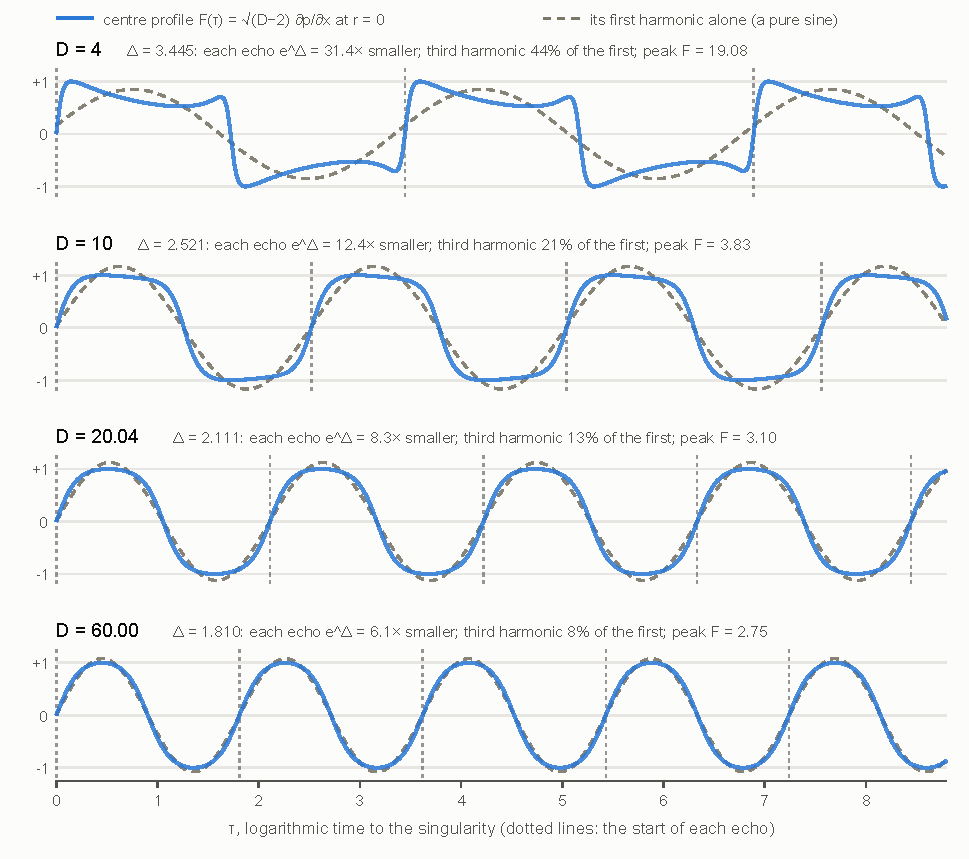
\includegraphics[width=0.92\linewidth]{figures/echo.pdf}
\caption{The echo across dimensions: the centre slope of the field,
$F(\tau) = \sqrt{D-2}\,\partial_x p$ at $r = 0$, over the same stretch of logarithmic time $\tau$ for $D = 4$, 10, 20
and 60, each scaled to its peak (dashed: its first harmonic). At $D = 4$ the profile is close to a square wave and
each echo is $e^{\Delta} = 31\times$ smaller than the last; at $D = 60$ it is nearly a pure sine and the factor is
$6.1$. The $D = 4$ profile is from the double-precision solver (39 harmonics); the others are double-double
solutions.}
\label{fig:echo}
\end{figure}

% =====================================================================================================
\section{Equations and numerical method}
\label{sec:method}

We use the self-similar radius $x$ (radius over time to the singularity, normalized so that the past light cone of
the singularity is at $x = 1$) and $\tau = -\ln(-t)$, or the phase $\theta = \omega\tau$ with $\omega = 2\pi/\Delta$.
With $n = D - 2$, $p$ and $m$ the (scaled) derivatives of the scalar field along the two radial null directions, $a$
the radial metric function ($b = a^2$) and $c$ the lapse-type function that sets the light cones, the equations are
\begin{align}
x c_x &= (n-1)\,c\,(b-1), &
x b_x &= b\,(p^2+m^2) - (n-1)\,b\,(b-1), \label{eq:E12}\\
x(x-c)\,p_x &= -\omega x\,p_\theta + G p - c p + \tfrac{n}{2}\,c\,(p+m), &
x(x+c)\,m_x &= -\omega x\,m_\theta - G m + c m - \tfrac{n}{2}\,c\,(p+m), \label{eq:E34}
\end{align}
with $G = (n-1)\,c\,(b-1)$, on $0 \le x \le 1$; $p$, $m$ contain only odd harmonics of $\theta$ and $b$, $c$ only even
ones; the solution is regular at $x = 0$, analytic at the past light cone $x = 1$, and $c(1) = 1$ fixes the gauge.

\emph{Double-precision solver} ($4 \le D \le 40$): spectral multiple shooting in $x$ with Fourier modes in $\tau$
(23--47 modes), with the integration-step error extrapolated out; near $D = 4$ the points are extrapolated in the
mode count. Above $D \approx 26$ the period is selected by an effect that weakens exponentially with $D$, and rounding
at $10^{-16}$ moves $\Delta$ by $10^{-7}$--$10^{-6}$ at $D = 30$--$40$.

\emph{Double-double solver} ($8.25 \le D \le 61.03$): double-double arithmetic (about 32 digits) on SIMD vectors;
Taylor series in $x$ of order 36 with truncation $10^{-32}$; centre and horizon series to $10^{-33}$; collocation in
$\tau$ on the half period (32 points); an exact Jacobian by forward-mode duals with a double-double LU; continuation in
$D$ with deflated Newton steps. The Jacobian has a ladder of near-null directions (high $\tau$-harmonics of the centre
data, singular values falling roughly like $e^{-0.7k}$); from $D = 35$ the centre harmonics above 13 are pinned, which
moves $\Delta$ by $5\times10^{-15}$ at $D = 35$ and $3\times10^{-17}$ at $D = 40$. Checks are listed in
Table~\ref{tab:checks}. The 857 points fit smooth curves to about $4\times10^{-15}$; the estimated error per point is
about $10^{-16}$ to $D = 60.1$ and a few $10^{-15}$ above, where the tolerance was relaxed.

\begin{table}[t]
\caption{Checks of the double-double solver.}
\label{tab:checks}
\begin{ruledtabular}
\begin{tabular}{ll}
Check & Result \\ \hline
double-double arithmetic against 40-digit mpmath & $1.3$--$1.6\times10^{-32}$ relative \\
horizon series against 40-digit mpmath & $2\times10^{-32}$ \\
Newton at $D = 8$ & quadratic, $|F| = 5\times10^{-31}$ in 4 steps \\
$\Delta(7)$, $\Delta(7.75)$ against 39-mode double-precision references ($\pm3\times10^{-11}$) & $+3.1\times10^{-12}$, $-2.8\times10^{-12}$ \\
32 / 48 / 64 collocation points in $\tau$, $D = 7$--$17$ & $\Delta$ agrees to $10^{-16}$ \\
32 / 48 collocation points, $D = 40$ & $9\times10^{-22}$ \\
harmonics pinned above 13 / above 15, $D = 40$ & $3\times10^{-17}$ \\
second machine (separate build), $D = 59.84$--$60.05$ & $2$--$4\times10^{-16}$ \\
32 points $D = 60.95$--$61.03$ against the $1/D$ fit on $D \le 60.1$ & $2.6\times10^{-15}$ \\
\end{tabular}
\end{ruledtabular}
\end{table}

% =====================================================================================================
\section{Results}
\label{sec:results}

\subsection{One formula for all $D \ge 4$}

With $\eps = 1/n = 1/(D-2)$,
\begin{equation}
\Delta(D) = \frac{\sum_{k=0}^{8} a_k \eps^k}{1 + b_1\eps + b_2\eps^2}, \qquad
\gamma(D) = \frac{\tfrac12 + \sum_{k=1}^{7} e_k \eps^k}{1 + f_1\eps + f_2\eps^2},
\label{eq:formula}
\end{equation}
with the coefficients of Table~\ref{tab:coef}, fitted on the double-precision points $4 \le D \le 30.2$. They reproduce
$\Delta$ to $5\times10^{-10}$ ($4 \le D \le 4.3$), $4\times10^{-9}$ ($4.3$--$20$) and $10^{-8}$ ($20$--$30$), and $\gamma$ to
$3.4\times10^{-7}$, $3.3\times10^{-8}$ and $2.3\times10^{-9}$, each within the precision of the points. Against the
double-double points, which the fit never saw, the formula holds to $2.7\times10^{-9}$ on $8.25$--$21$,
$7.5\times10^{-9}$ to $D = 30$ and $5.8\times10^{-8}$ to $D = 61$ (Fig.~\ref{fig:delta}). The limit $\gamma_\infty = 1/2$ is
imposed in the $\gamma$ fit, not derived; unconstrained fits on $D \ge 8$--$12$ give $0.4996$--$0.4998$. The denominators
vanish only at $D = -3.2, -11.0$ ($\Delta$) and $D = -13.3, -20.4$ ($\gamma$). Values are listed in Table~\ref{tab:values}.

\begin{table}[t]
\caption{Coefficients of Eq.~\eqref{eq:formula}.}
\label{tab:coef}
\begin{ruledtabular}
\begin{tabular}{rllll}
$k$ & $a_k$ & $b_k$ & $e_k$ & $f_k$ \\ \hline
0 & $+1.6438975180$ & $1$ & $+0.5$ (fixed) & $1$ \\
1 & $+4.0378045077\times10^{1}$ & $+1.8251453626\times10^{1}$ & $+1.8083629635\times10^{1}$ & $+3.7683686025\times10^{1}$ \\
2 & $+2.5233285989\times10^{2}$ & $+6.8182050167\times10^{1}$ & $+1.5241588758\times10^{2}$ & $+3.4245505235\times10^{2}$ \\
3 & $+2.0673502321\times10^{2}$ & & $-5.2341588541\times10^{1}$ & \\
4 & $-3.5709850575\times10^{2}$ & & $+9.9259594505$ & \\
5 & $+3.1347320996\times10^{2}$ & & $-9.8386450353\times10^{1}$ & \\
6 & $-4.1891374574\times10^{2}$ & & $+7.4529506074\times10^{1}$ & \\
7 & $+3.2695252782\times10^{2}$ & & $-4.8272358903\times10^{1}$ & \\
8 & $-1.6050467699\times10^{2}$ & & & \\
\end{tabular}
\end{ruledtabular}
\end{table}

\begin{table}[t]
\caption{Values. $\Delta$ for $D = 10$--$60$ is double-double (interpolated to $10^{-14}$ where $D$ is not a computed
point); $\Delta(8)$ is a separate double-double run; $\Delta$ for $D = 4$--$7$ and $\gamma$ to $D = 40$ are
double-precision; $\gamma(50)$, $\gamma(100)$, $\gamma(1000)$ are formula values. $\Delta(70)$ and $\Delta(100)$ are
extrapolations on which all models fitting the double-double points agree (to $10^{-11}$, $2\times10^{-8}$);
$D = 1000$ and $\infty$ assume analyticity in $1/D$.}
\label{tab:values}
\begin{ruledtabular}
\begin{tabular}{rll|rll}
$D$ & $\Delta$ & $\gamma$ & $D$ & $\Delta$ & $\gamma$ \\ \hline
4 & 3.4454524 & 0.3739610 & 20 & 2.112080154580 & 0.4737107 \\
5 & 3.2217019 & 0.4131269 & 30 & 1.964957899258 & 0.4807927 \\
6 & 3.0094832 & 0.4300795 & 40 & 1.888568197910 & 0.484776 \\
7 & 2.8427532 & 0.4399912 & 50 & 1.841659503007 & 0.48736 \\
8 & 2.711790054444 & 0.4467164 & 60 & 1.809889459975 & \\
10 & 2.521078919562 & 0.4555879 & 70 & 1.78693476494 & \\
12 & 2.389188553641 & 0.4614056 & 100 & 1.7450264844 & 0.49313 \\
15 & 2.253098407194 & 0.4673656 & 1000 & 1.65424086 & 0.4992 \\
 & & & $\infty$ & $1.64389375 \pm 10^{-8}$ & $1/2$ (assumed) \\
\end{tabular}
\end{ruledtabular}
\end{table}

\begin{figure}[t]
\centering
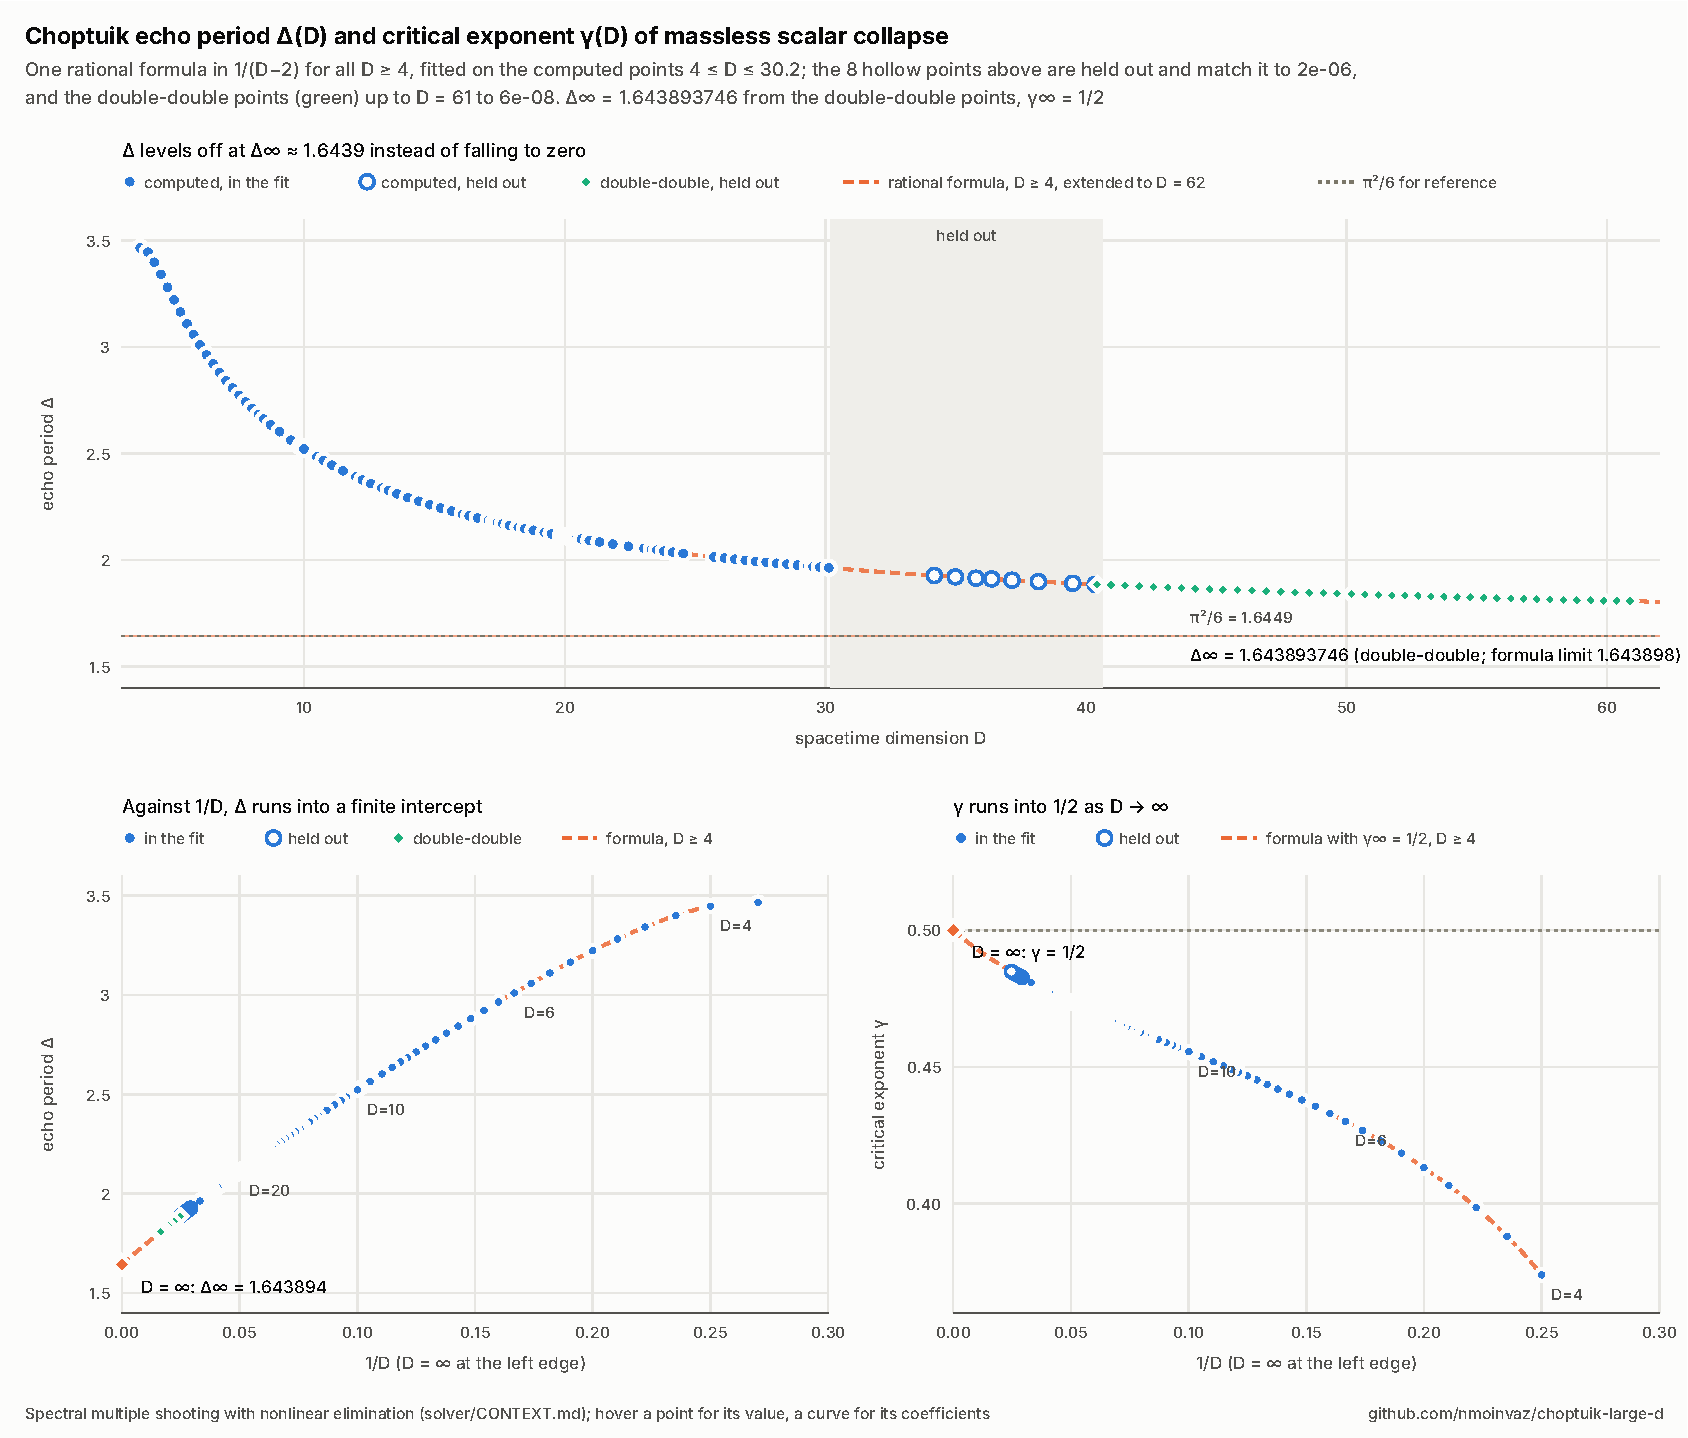
\includegraphics[width=\linewidth]{figures/delta.pdf}
\caption{$\Delta(D)$ and $\gamma(D)$ with the rational formula~\eqref{eq:formula} (dashed), fitted on
$4 \le D \le 30.2$; hollow points are held out, and green diamonds are double-double points up to $D = 61$.}
\label{fig:delta}
\end{figure}

\subsection{Comparison with published values}

At $D = 4$ the formula gives $\Delta = 3.4454524$ and $\gamma = 0.3739610$, in agreement with
$\Delta = 3.445452402(3)$~\cite{MartinGarciaGundlach2003} to about $10^{-8}$ and with
$\gamma = 0.373961 \pm 10^{-6}$~\cite{EckerEtAl2026} to about $10^{-7}$. Below $D = 4$ a cubic through the 47-mode
double-precision points at $D = 3.70$--$3.80$ puts the maximum of $\Delta$ at $D = 3.75570$, $\Delta = 3.466774$, in
agreement to $2\times10^{-6}$ with $D = 3.755726$, $\Delta = 3.466772$ of~\cite{EckerEtAl2026}.

At $D = 5$, Ref.~\cite{EckerEtAl2026} gives $\Delta = 3.22176$ and $\gamma = 0.41322$, which are $5.8\times10^{-5}$ and
$9.3\times10^{-5}$ above our $3.2217019$ and $0.4131269$. Ours are stable across 31, 39 and 47 Fourier modes to about
$10^{-7}$, and Bland and Kunstatter give $\gamma(5) = 0.4131 \pm 0.0001$~\cite{BlandKunstatter2007}, matching ours.
The cause of the discrepancy is not known; an independent recomputation is in progress. Below $D = 4$, $\gamma$
extrapolated from our 47-mode points suggests $\gamma(3.5) \lesssim 0.33$, against $0.349 \pm 0.003$
in~\cite{BlandEtAl2005}; our points there are under-resolved, and this is an open check.

\subsection{Physical reading}

Each echo is a factor $e^{\Delta}$ smaller than the last: 31 at $D = 4$, 12 at $D = 10$, 5.2 at $D = \infty$. A
near-critical collapse makes about $\gamma\ln(1/|p-p^*|)/\Delta$ echoes, so each further echo costs
$\Delta/(\gamma\ln10)$ decimal digits of fine-tuning: 4.0 at $D = 4$, 2.4 at $D = 10$ and 1.43 at $D = \infty$. At large
$D$ the field and its gravity weaken: the centre slope of the field falls like $2.72/\sqrt n$ and the departure of $c$ from
1 at the centre like $3.65/n$ (Sec.~\ref{sec:theory}).

% =====================================================================================================
\section{The large-$D$ limit}
\label{sec:limit}

\subsection{Is the period analytic in $1/D$?}

Each model in Table~\ref{tab:analytic} is a polynomial in one variable, fitted at 60 digits on the cleaned
double-double points $10 \le D \le 45$ (or $\le 37.5$) and compared with every point above, up to $D = 60.1$, which it
never saw (the data snapshot when the table was made; Fig.~\ref{fig:heldout} uses all points to $D = 61.0$). Every
model fits its range to the level of the points; the unseen points decide. Fitted on $D \le 45$, the $1/D$ series
predicts $\Delta$ fifteen units of $D$ ahead to $5\times10^{-13}$, while the series in half-integer powers miss by 40 to
300 times more, and their limits jump with the degree. Adding one non-analytic term ($D^{-1/2}$, $D^{-3/2}$,
$\ln D/D$, $\ln D/D^2$ or $e^{-D/4}$) to the degree-16 series changes neither the prediction nor the limit, and the
term's coefficient is not determined.

\begin{table}[t]
\caption{Held-out test of large-$D$ models (cleaned double-double points; snapshot $D \le 60.1$).}
\label{tab:analytic}
\begin{ruledtabular}
\begin{tabular}{lllll}
Model & max residual, $10 \le D \le 45$ & worst error, $45 < D \le 60.1$ & fitted on $D \le 37.5$: worst error & limit \\ \hline
$1/D$, degree 16 & $4.1\times10^{-15}$ & $5.2\times10^{-13}$ & $4.2\times10^{-11}$ & 1.64389375 \\
$1/D$, degree 18 & $4.0\times10^{-15}$ & $1.8\times10^{-12}$ & $1.5\times10^{-10}$ & 1.64389377 \\
$1/(D-2)$, degree 18 & $4.0\times10^{-15}$ & $2.8\times10^{-12}$ & $7.9\times10^{-11}$ & 1.64389377 \\
$(D-2)^{-1/2}$, degree 20 & $3.9\times10^{-15}$ & $2.0\times10^{-11}$ & $3.9\times10^{-10}$ & 1.636 \\
$D^{-1/2}$, degree 20 & $3.8\times10^{-15}$ & $1.6\times10^{-10}$ & $6.2\times10^{-9}$ & 1.547 \\
\end{tabular}
\end{ruledtabular}
\end{table}

\begin{figure}[t]
\centering
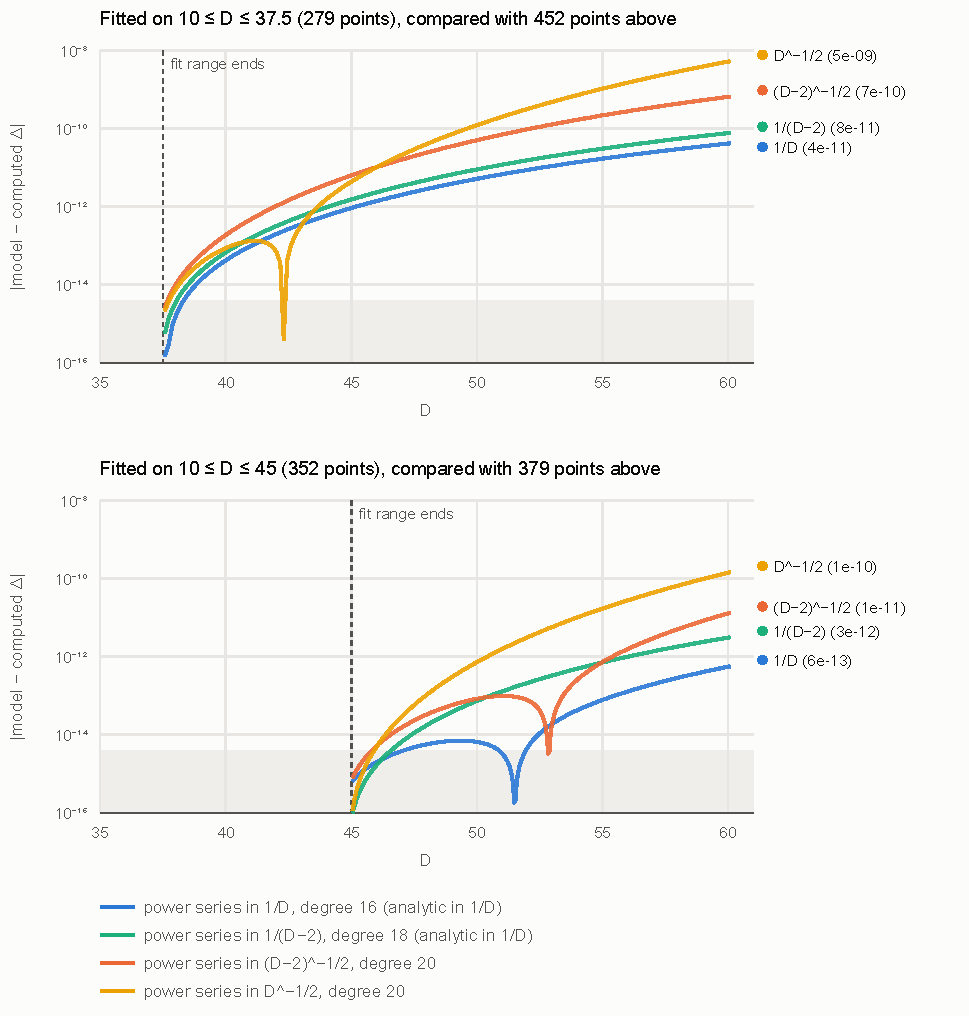
\includegraphics[width=0.8\linewidth]{figures/heldout.pdf}
\caption{$|\text{model} - \text{computed}\ \Delta|$ on every double-double point above the fitted range, for fits on
$10 \le D \le 37.5$ (top) and $10 \le D \le 45$ (bottom); shaded: the level of the points.}
\label{fig:heldout}
\end{figure}

Fitted on all cleaned points, power series in $1/D$ of degree 16--20 and in $1/(D-2)$ of degree 18--20 fit to the
noise and give limits from $1.643893744$ to $1.643893752$ (snapshot $D \le 60.1$) and from $1.643893745$ to
$1.643893752$ (all 823 cleaned points to $D = 61.03$). Hence, if $\Delta$ is analytic in $1/D$,
\begin{equation}
\Dinf = 1.64389375 \pm 10^{-8}, \qquad \omega_\infty = 2\pi/\Dinf = 3.82213589 \pm 2\times10^{-8},
\end{equation}
and $\Delta(D) \approx \Dinf + 10.37/n + \dots$. The analytic form is the natural default but not proven: as shown in
Sec.~\ref{sec:theory}, the period is selected by an effect the $1/D$ expansion does not see.

\subsection{The conjecture $\Delta \to 0$}

The conjecture $\Delta \to 0$~\cite{EckerEckerGrumiller2026,EckerEtAl2026} comes with no rate. Fitted on
$10 \le D \le 45$ and compared with $45 < D \le 61$: a power-law approach to 0, $D^{-p}$ times a series in $1/D$ with
$p \ge 0.01$, misses the held-out points by $6\times10^{-8}$ or more, against $7\times10^{-13}$ for the analytic series;
a series in $1/\ln D$ with zero limit misses them by $1.3\times10^{-11}$ and still gives $\Delta \approx 0.88$ at
$D = 10^{30}$; adding a $c/\ln D$ term to the analytic series gives $c \approx 4\times10^{-7}$ and leaves the limit at
$1.6438937$. A power-law approach to 0 is excluded; a logarithmic one is disfavoured but cannot be excluded from
$D \le 61$ alone. Bland's hypothesis $\Dinf = 5/2$~\cite{Bland2007} is excluded by $\Delta(14) = 2.29$ and decreasing.

\subsection{Candidate closed forms}

Nine closed forms were forced as the limit of a power series in $1/D$ fitted on $10 \le D \le 45$ (degree 14 to 26) and
compared with the 351 cleaned points from 45 to 59.8 (Table~\ref{tab:cand}). The closest sits $1.3\times10^{-5}$ from
the limit, more than 1000 times its uncertainty, and every forced fit predicts the unseen points at least 100 times
worse than the free fit. A search over products of standard constants and Bessel zeros finds nothing in
$1.6438936$--$1.6438939$, nor in a window about 27 times wider. Whether $\Dinf$ has a closed form is open.

\begin{table}[t]
\caption{Candidate closed forms for $\Dinf$, forced as the limit: best held-out error and its ratio to the free fit.
$G$ is Catalan's constant, $j_{\nu,k}$ the $k$-th zero of $J_\nu$.}
\label{tab:cand}
\begin{ruledtabular}
\begin{tabular}{llll}
Candidate & value & minus $\Dinf$ & held-out error (ratio) \\ \hline
none (free fit) & $1.64389375 \pm 10^{-8}$ & & $4.7\times10^{-13}$ \\
$\tfrac57\sqrt{G}\,j_{0,1}$ & 1.6439747 & $+8.1\times10^{-5}$ & $6.2\times10^{-11}$ (130) \\
$\tfrac75(\ln2)^{-2}\pi^{-1/2}$ & 1.6440014 & $+1.1\times10^{-4}$ & $1.1\times10^{-10}$ (220) \\
$\tfrac72\sqrt{\ln2/\pi}$ & 1.6440152 & $+1.2\times10^{-4}$ & $1.3\times10^{-10}$ (270) \\
$\tfrac98\sqrt{j_{2,1}/j_{0,1}}$ & 1.6440207 & $+1.3\times10^{-4}$ & $1.4\times10^{-10}$ (290) \\
$\tfrac{10}{9}\sqrt{j_{0,1}/\ln3}$ & 1.6439063 & $+1.3\times10^{-5}$ & $5.4\times10^{-11}$ (110) \\
$\pi^2/6$ & 1.6449341 & $+1.0\times10^{-3}$ & $1.7\times10^{-9}$ (3500) \\
$2\pi/j_{1,1}$ & 1.6397878 & $-4.1\times10^{-3}$ & $7.0\times10^{-9}$ (15000) \\
$\sqrt e$ & 1.6487213 & $+4.8\times10^{-3}$ & $8.1\times10^{-9}$ (17000) \\
$(1+\sqrt5)/2$ & 1.6180340 & $-2.6\times10^{-2}$ & $4.4\times10^{-8}$ (92000) \\
\end{tabular}
\end{ruledtabular}
\end{table}

% =====================================================================================================
\section{Large-$D$ theory}
\label{sec:theory}

\subsection{Scaling}

On the double-double solutions at $D = 12$--$60$: $p \approx x F(\theta)/\sqrt n$ near the centre and $p + m$ is
smaller by a further factor of order $1/n$; $c = 1 - O(1/n)$ and $b - 1 = (p^2+m^2)/(n-1)$ to about 3\%; and the
centre series has the exact symmetry $m(x) = p(-x)$. The first harmonic of $F = \sqrt n\,\partial_x p(0)$ falls from
3.480 at $D = 20$ to 2.962 at $D = 60$ and extrapolates to about 2.72; $n(1 - \langle c(0)\rangle)$ and $\langle F^2\rangle$
approach a common limit near 3.7.

\subsection{The $1/n$ expansion never fixes the period}

Write $p = \eps^{1/2}P$, $m = \eps^{1/2}M$, $S = P + M$, $\Delta_P = P - M$, and expand $S = \sum_{k\ge1}\eps^kS_k$,
$\Delta_P = \sum_{k\ge0}\eps^kD_k$, $c = 1 - \sum_{k\ge1}\eps^kG_k$, $b = 1 + \sum_{k\ge2}\eps^kB_k$,
$\omega = \sum_k\eps^k\omega_k$ (integer powers of $\eps$; this is the scaling measured above, and the statements below
hold within this ansatz).

\begin{proposition}\label{prop:1}
Let $F(\theta)$ be any smooth $2\pi$-periodic function with odd harmonics only, $\omega_0, \omega_1, \dots$ any numbers
and $K_1(\theta), K_2(\theta), \dots$ any smooth odd-harmonic functions. Then there is exactly one formal solution with
$D_0 = 2xF$ in which, at every order, $S_k$ is an even polynomial in $x$ starting at $x^2$, $D_k - xK_k$ is an odd
polynomial starting at $x^3$, and $G_k$, $B_{k+1}$ are even polynomials ($B$ starting at $x^2$) with $G_k(1) = 0$. Every
order is regular at the centre and analytic at the light cone.
\end{proposition}

\emph{Proof sketch.} Induction on $k$. The $b$ equation gives $B_{k+1}$ algebraically (its coefficient is
$(n-1)b \approx 1/\eps$); the $c$ equation gives $-x\partial_xG_k \in x^2E$ ($E$: even polynomials with periodic
coefficients), so $G_k$ is an even polynomial without $\log x$, fixed by $G_k(1) = 0$; the difference equation gives
$S_k \in x^2E$; and the sum equation reads $x\partial_xD_k - D_k = R_k$ with $R_k$ odd and starting at $x^3$, because
$x\partial_x - 1$ annihilates $xK_j$. The only possible obstruction, an $x^1$ term in $R_k$ that would produce $x\log x$,
never occurs. Parity in $x$ and the harmonic content in $\theta$ are preserved at each step. Polynomials are analytic
at $x = 1$, and nothing constrains $F$ or the $\omega_k$. $\square$

The first orders (sympy, to fourth order) are $P_0 = xF$, $B_2 = 2x^2F^2$, $G_1 = F^2(1-x^2)$,
$S_1 = 2x^2(F + \omega_0F')$ and $D_1 = x^3(\omega_0^2F'' + 3\omega_0F' + 2F - 2F^3) + xK_1$. Substituting the expansion
through $S_3$, $G_3$, $B_4$ into the exact equations with $F$ from the $D = 60$ solution, the relative residuals fall
like $n^{-3}$ for $n = 50$--$800$, both for $\omega_0 = 2\pi/1.64389$ and for a wrong $\omega_0 = 2\pi/1.4$.

So if $\Delta(D)$ is analytic in $1/D$, its expansion coefficients cannot be computed order by order from the field
equations: the selection works through terms smaller than any power of $1/n$. The same holds for the critical
exponent: the expansion of growing perturbations $e^{\lambda\tau}$ goes through for any $\lambda$ (the same induction
with $\partial_\tau \to \lambda + \omega\partial_\theta$; checked with sympy through order 2), so $\gamma = 1/\lambda$ is also
selected beyond all orders.

\subsection{The leading-order problem}

At leading order ($c = b = 1$) the equations describe a free wave in self-similar form. For one harmonic
$e^{i\mu\theta}$ put $s = i\mu\omega$, $\alpha = (1+s)/2$, $\beta = (2+s)/2$, $\kappa = (n+1)/2$.

\begin{proposition}\label{prop:2}
The solution regular at the centre is, up to a constant, $p - m = x\,{}_2F_1(\alpha,\beta;\kappa;x^2)$. Near the light
cone it contains the non-analytic branch $(1-x^2)^{n/2-1-s}$ with coefficient
\begin{equation}
C(n,s) = \frac{\Gamma\!\left(\frac{n+1}{2}\right)\Gamma\!\left(s+1-\frac n2\right)}{\Gamma\!\left(\frac{1+s}{2}\right)\Gamma\!\left(\frac{2+s}{2}\right)},
\label{eq:C}
\end{equation}
which is finite and non-zero for every real $\omega \ne 0$, odd $\mu$ and $n \ge 2$. Hence no time-periodic
self-similar solution of the linear problem is analytic at the light cone, for any $D \ge 4$.
\end{proposition}

\emph{Proof sketch.} Eliminating $p+m$ gives Gauss's equation for $y = x\,w(x^2)$; regularity (for $n = 2$, parity)
selects ${}_2F_1(\alpha,\beta;\kappa;z)$, and the connection formula~\cite{AbramowitzStegun} applies because
$\kappa - \alpha - \beta = n/2 - 1 - s$ is not an integer; its second coefficient is $C(n,s)$, a ratio of Gamma functions
whose arguments have non-zero imaginary parts. $\square$

For the fundamental at $\omega = \omega_\infty$, $|C| = 0.0121$, 0.0114, 0.0124, 0.0192, 0.0405 at $n = 18$, 38, 58, 200,
1000. The free wave equation in similarity coordinates was analysed in 3+1 dimensions by Donninger~\cite{Donninger2008};
the leading-order freedom of the large-$D$ problem is also noted in~\cite{EckerEckerGrumiller2026}.

\subsection{What gravity does to the non-analytic piece}

The non-analytic piece is a fast WKB mode; in Proposition~\ref{prop:2} it is $x^{2-n}(1-x^2)^{n/2-1-s}$.

\begin{proposition}\label{prop:3}
Let $c = 1 - \eps F^2(1-x^2) + O(\eps^2)$ as in Proposition~\ref{prop:1}, and
$\Phi(x) = \ln x - \tfrac12\ln(1-x^2)$. Perturbations
$\delta p = e^{-n\Phi}(A + O(1/n))$, $\delta m = e^{-n\Phi}\big(\tfrac{1-x}{1+x}A + O(1/n)\big)$ solve the linearized
equations on $0 < x < 1$ to this order if and only if
\begin{equation}
x(1-x^2)\,\partial_xA - 2\omega x^2\,\partial_\theta A = (1 + x - 2x^2F^2)\,A ,
\end{equation}
i.e.\ along the characteristics $\theta = \theta_0 + \omega\ln(1-x^2)$,
$A = A_0(\theta_0)\,\frac{x}{1-x}\exp\!\big(-\int_0^x \frac{2tF(\theta_0 + \omega\ln(1-t^2))^2}{1-t^2}\,dt\big)$.
\end{proposition}

\emph{Proof sketch.} The order-$n$ terms give $x(1-x^2)\Phi' = 1$ and $\delta m/\delta p = (1-x)/(1+x)$; at order 1 the
corrections satisfy a singular linear system whose left null vector $(1+x, -(1-x))$ gives the transport equation as the
solvability condition. Perturbations of $b$, $c$ and $G\,\delta p$ enter one order later (confirmed symbolically from the
exact equations). $\square$

Integrating the linearized equations directly from $x = 0.9$ to $0.72$ ($F = 2.72\sin\theta + 0.22\sin3\theta$,
$\omega = \omega_\infty$) reproduces the transported $A$ with relative errors $0.57$, $0.26$, $0.13$, $0.062$, $0.031$ at
$n = 100$--$1600$, i.e.\ like $1/n$; with the full $O(1/n)$ background the numbers are nearly the same. Three
consequences: (i) gravity acts on the non-analytic piece at order 1 (over this interval it multiplies it by about 40),
and shifts the light-cone exponent by $\langle F^2\rangle \approx 3.7$, so an expansion in the wave amplitude is not a route
to the selection; (ii) the factor never vanishes, so gravity cannot cancel the piece on the way to the light cone;
(iii) every characteristic reaches $x = 0$, where the fast mode is the singular branch $x^{2-n}$, so a regular solution
carries no fast mode on $0 < x < 1$ at any order of this WKB expansion. The non-analytic piece must come from a Stokes
phenomenon.

\subsection{The light-cone coefficient as a Stokes multiplier}

\begin{proposition}[derivation]\label{prop:4}
Let $y(\eps) = x\,{}_2F_1(\alpha,\beta;\kappa;z)$ with $z = x^2$, $\kappa = (1 + 1/\eps)/2$, and $y \sim \sum_k y_k\eps^k$.
Then
\begin{equation}
y_k = 2x(-1)^{k-1}\sum_{J\ge0}R_J(2J+1)^{k-1}, \qquad
R_J = \frac{(-1)^J(\alpha)_{J+1}(\beta)_{J+1}}{J!\,(J+1)!}\,z^{J+1}{}_2F_1(\alpha+J+1,\beta+J+1;J+2;z),
\end{equation}
convergent for $x < 1/\sqrt2$ and continued above, and as $k \to \infty$
$y_k \approx \sum_\ell K_\ell(x)\,\Gamma(k+s+\tfrac12)/\big(\Phi(x) + i\pi(\ell+\tfrac12)\big)^{k+s+1/2}$, dominated by
$\ell = -1$, i.e.\ by the singulant $\chi = \Phi - i\pi/2$.
\end{proposition}

The first formula is the pole expansion of ${}_2F_1$ in $\kappa$; the second follows from the large-$J$ form of $R_J$ and
Poisson summation over $J$. This is a derivation, not a proof: a full proof needs a growth bound for the pole expansion,
the exchange of the $J$-sum with the expansion of $1/(1+(2J+1)\eps)$, error bounds inside the Poisson sum, control of
the continuation to $x > 1/\sqrt2$, and the branch of $\chi^{k+s+1/2}$. Numerically, the pole sum equals the direct series
to $10^{-49}$--$10^{-91}$; the late orders computed to order 122 at 90 digits give $\chi = \Phi - i\pi/2$ to
$3$--$7\times10^{-3}$ at $x = 0.7$--$0.9$; and the predicted Dingle constant
$K = e^{-i\pi(1+s)}\,2^{-s-1/2}/(\Gamma(\alpha)\Gamma(\beta))$, with prefactor $x^2(1-x^2)^{-1-s}$ and exponent
$g = -(s+\tfrac12)$~\cite{Dingle1973}, is matched to $6\times10^{-4}$ at $x = 0.9$.

Hence: $e^{-n\chi} = e^{in\pi/2}x^{-n}(1-x^2)^{n/2}$ is the fast mode of Proposition~\ref{prop:3}; $\chi$ vanishes only
at $x = \infty$, so the mode is born at the outer singular point; its Stokes line is the real axis $x > 1$ approached
from above, where $\chi = \ln(x/\sqrt{x^2-1})$; on $0 < x < 1$ nothing is switched on (the optimally truncated series
matches the exact solution to $4\times10^{-40}$ at $x = 0.9$, $n = 60$, against a singular-branch size of
$7\times10^{-21}$). The Stokes line ends at the light cone, and $C(n,s)$ is the Stokes multiplier.

\subsection{The inner problem}
\label{sec:inner}

At $x \sim \sqrt n$ the expansion is not uniform: gravity is of order one and fast and slow modes are not separated.
With $\xi = x/\sqrt n$, $y = p - m$, $\sigma = \sqrt n\,(p+m)$, $b - 1 = \eta/n$ and
$L = \xi^2\partial_\xi + \omega\xi\partial_\theta$, the equations become, at leading order,
\begin{equation}
L\,y = c\,\sigma, \qquad L\,\sigma = c\,\xi\,\partial_\xi y + c\,(\tfrac12y^2 - 1)\,y, \qquad
\xi\,\partial_\xi c = \tfrac12\,c\,y^2, \qquad \eta = \tfrac12y^2,
\end{equation}
with no large parameter left. Its formal solution regular at $\xi = 0$ reproduces the top-degree coefficients of the
outer polynomials of Proposition~\ref{prop:1} (checked to $2\times10^{-13}$ at orders 1--10). Without gravity, with
$t = 1/\xi$ and $w = t^{-s}y$ along characteristics, it reduces to Hermite's (Weber's) equation; the regular solution is
$y = 2\xi\,{}_2F_0(\alpha,\beta;;2\xi^2)$, whose Stokes constant gives, by the duplication formula,
\begin{equation}
C(n,s) \approx -\,i\,\frac{\sqrt{2\pi}}{\Gamma(1+s)}\,(n+1)^{s+1/2}\,e^{-i\pi\Lambda}\,\big(1 + O(s^2/n)\big), \qquad \Lambda = \tfrac n2 - 1 - s,
\end{equation}
Weber's classical Stokes constant~\cite{DLMF}; the ratio to the exact~\eqref{eq:C} is $1.00014$ at $n = 10^5$ ($\mu = 1$).

\emph{Working hypothesis.} With gravity, the selection rule at $D = \infty$ is that the fast-type Stokes multipliers of the
formal inner solution vanish, one complex condition per odd harmonic; the unknowns are $F$'s harmonics and $\omega$, so
the count balances. This is derived from the matching but not proved. In the inner region the fast mode obeys
$\xi\partial_\xi a + 2\omega\partial_\theta a = 2F^2a$ (the large-$x$ limit of Proposition~\ref{prop:3}); the Borel
singularity stays at $\zeta = \tfrac12$ and the exponents shift by $\langle F^2\rangle$.

\emph{Computations with gravity.} Two independent implementations (lateral solutions on either side of the Stokes
line, and Borel--Darboux fits in ball arithmetic) reproduce the linear constant to $10^{-11}$ and $6\times10^{-27}$. With
$F = A\sin\theta$ alone, both find an isolated zero of the multiplier at $A = 2.542148$, $\omega = 2.969777$; it is not the
physical solution ($\omega$ 22\% low) and does not survive adding harmonic 3. Truncating harmonics is not a controlled
approximation here: the linear multipliers grow like $F_\nu e^{\pi|\nu|\omega/2}$.

\emph{Amplitude expansion.} Writing $F = A\sin\theta + \sum_{\nu\ge3} f_\nu(A)e^{i\nu\theta}$ (plus c.c.), harmonic $\mu$
first appears at order $A^{|\mu|}$, so every harmonic is kept exactly. Tuning $f_\nu$ order by order so that the
multipliers of all harmonics $|\nu| \ge 3$ vanish, at $A = 2.72$ and $\omega = \omega_\infty$, gives
$|F_3/F_1| = 0.055$ and $|F_5/F_1| = 0.0030$, with ratios $f_{\nu+2}/f_\nu \approx qA^2$, $|q|A^2 \approx 0.063$, nearly
independent of $\nu$. The double-double solutions at $D = 20$--$60$, extrapolated in $1/n$ (degree 2--3), give
$|F_3/F_1| \to 0.0552$--$0.0549$ and $|F_5/F_1| \to 0.0034$--$0.0032$, and the ratios $|F_{\nu+2}/F_\nu|$
($\nu = 1,\dots,9$) extrapolate to $0.055$--$0.072$, a finite decay rate of 1.3--1.45 per harmonic, as predicted
(Fig.~\ref{fig:spectrum}; the extrapolations are not fully converged). This is the first number the inner problem has
produced that can be checked against the solutions, and it agrees. The harmonic-1 condition, which would fix $\omega$ and
hence $\Dinf$, is still open: its series $S_1/S_1^{(1)} = 1 + \sigma_1A^2 + \sigma_2A^4 + \dots$ is known to four terms
($\sigma_1 = 0.7436 + 0.5245i$, $\sigma_2 = 0.1188 + 0.3981i$, $\sigma_3 = -0.0540 + 0.1166i$, $\sigma_4 \approx -0.029 + 0.011i$),
which do not locate its zero; an extended-precision computation is in progress.

\begin{figure}[t]
\centering
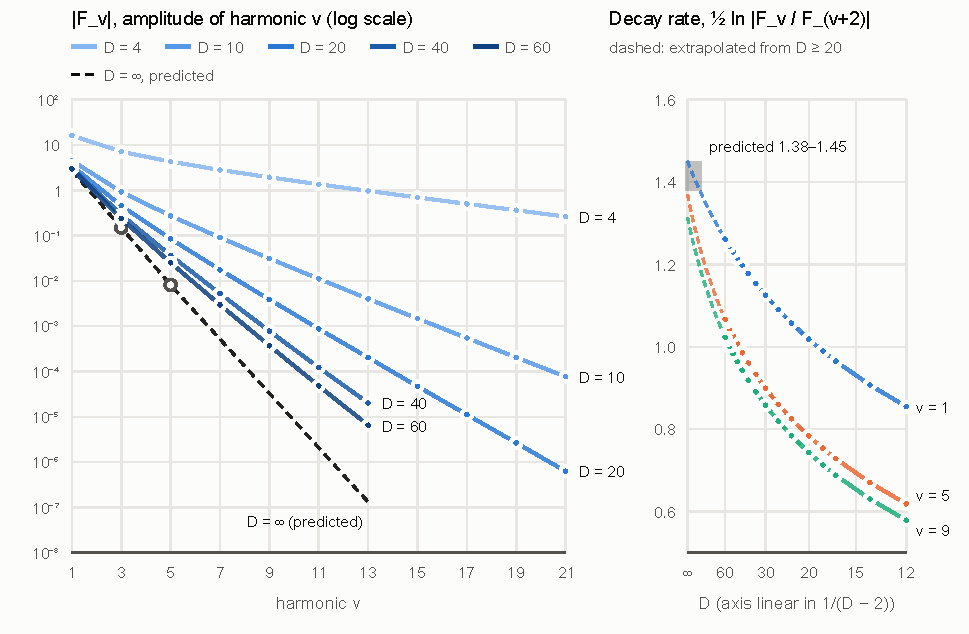
\includegraphics[width=\linewidth]{figures/spectrum.pdf}
\caption{Left: amplitude $|F_\nu|$ of each odd harmonic of the echo profile for $D = 4$--$60$ and the $D = \infty$
prediction of the inner problem (dashed; beyond $\nu = 5$ the leading-order ratio, conjectured). Right: the decay rate
per harmonic, $\frac12\ln|F_\nu/F_{\nu+2}|$, against $1/(D-2)$, with extrapolations from $D \ge 20$ and the predicted
$D = \infty$ band.}
\label{fig:spectrum}
\end{figure}

\emph{The critical exponent.} In the inner problem two growth rates are exact, from symmetries: $\lambda = 0$ (a shift of
$\theta$) and $\lambda = 1$ (a shift of the time of the singularity, the $D = \infty$ limit of the gauge mode); no symmetry
gives $\lambda = 2$. Free fits of the data give $\gamma_\infty = 0.4996$--$0.4998$; why $\lambda_\infty = 2$ to $10^{-3}$ is
open.

\subsection{Relation to the next-to-leading-order condition of Ref.~\cite{EckerEckerGrumiller2026}}
\label{sec:eeg}

Ecker, Ecker and Grumiller use the same gauge: their $f = \alpha/a$ is our $c$, with $f = 1$ at the self-similarity horizon
$x = 1$, and their profile is $\beta(\tau) \approx \sqrt{2/n}\,F(\omega\tau)$. At next-to-leading order they require
$f \le 1$ near the horizon at the zeros of $\beta$, which gives their Eq.~(20); in our variables,
$\omega^2F'' + 3\omega F' = 0$ at the zeros of $F$. Within our framework this condition does not select $\Delta$, for the
following reasons. The inequality $f \le 1$ holds for every regular solution, whatever the period: from
$xb_x = b(p^2+m^2) - (n-1)b(b-1)$ with $b(0) = 1$, $b$ can never drop below 1, so $xc_x = (n-1)c(b-1) \ge 0$ and
$c \le c(1) = 1$. In the formal family of Proposition~\ref{prop:1}, near a zero of $F$,
\begin{equation}
b - 1 = 2\eps^2x^2F(\theta - \delta\theta)^2 + 2\eps^4\omega^2x^4F'^2 + \dots, \qquad
\delta\theta(x) = -\eps\omega x^2\,\frac{3F' + \omega F''}{2F'},
\end{equation}
so the next-to-leading-order term is the cross term of a square whose square term arrives one order later; the
discriminant $16\omega^2x^6F'^4$ is positive for every $F$ and $\omega$. The double-double solutions are consistent with
this: they violate Eq.~(20) [$(\omega^2F''+3\omega F')/(3\omega F') = 0.98$--$1.06$ at $D = 12$--$60$, since $F$ is nearly
antisymmetric about its zeros], the zero line of $p - m$ tilts as $\delta\theta(x)$ predicts (measured over predicted at
$x = 1$: 0.69 to 0.88 for $D = 20$--$60$), and the maximum of $c$ at the centre approaches $1 - (\eps^3/2)\omega^2F'^2$,
their Eq.~(22) in this scaling (ratio 0.36 to 0.86).

% =====================================================================================================
\section{Discussion}

The numerics give $\Delta(D)$ to high precision up to $D = 61$, and they favour a finite limit
$\Dinf = 1.64389375$ strongly, under the assumption of analyticity in $1/D$ that they support but cannot prove. The
theory explains why that number cannot come from the $1/D$ expansion: the expansion is unobstructed for every period,
and the selection acts through an exponentially small, Stokes-type effect whose linear version is solved exactly. The
inner problem at $x \sim \sqrt n$ is $n$-free; its higher-harmonic conditions already reproduce the shape of the echo
at $D = \infty$. Open are: the harmonic-1 condition of the inner problem, which would give $\Dinf$ (and possibly a closed
form) from first principles; a proof of the working hypothesis; the value $\lambda_\infty = 2$; the $D = 5$ discrepancy;
and the behaviour just below $D = 4$.

\section{How this work was done}
\label{sec:how}

N.~M. chose the problem, set the direction at each step and ran the long computations on his own machine. The code, the
computations, the derivations, the proofs and the text, including this paper, were produced by Claude, Anthropic's AI
model, working as a set of coordinated agents. N.~M. has not checked the mathematics himself, and no human expert has
reviewed the work. Checks made: two independent solvers agree where they overlap; two machines with separate builds
agree to $2$--$4\times10^{-16}$; every fit table reproduces from the data with the stated command; Propositions 1--3
and the inner equations were re-derived by separate agents (with sympy where possible); the inner Stokes multiplier was
computed by two implementations that share no code; values at $D = 4$ and the maximum of $\Delta$ agree with the
literature; and an independent agent refereed the write-up. Corrections are welcome.

\emph{Data and code.} All data, code and derivation scripts are at
\url{https://github.com/nmoinvaz/dss-residual-kernel}, with a reproduction script (\texttt{reproduce.sh}) and the
double-double points in \texttt{hp/data/delta\_dd.csv}.

\begin{thebibliography}{99}
\bibitem{Choptuik1993} M. W. Choptuik, Phys.\ Rev.\ Lett.\ \textbf{70}, 9 (1993).
\bibitem{Gundlach1997} C. Gundlach, Phys.\ Rev.\ D \textbf{55}, 695 (1997), arXiv:gr-qc/9604019.
\bibitem{MartinGarciaGundlach2003} J. M. Mart\'in-Garc\'ia and C. Gundlach, Phys.\ Rev.\ D \textbf{68}, 024011 (2003),
arXiv:gr-qc/0304070.
\bibitem{GundlachReview2025} C. Gundlach, D. Hilditch and J. M. Mart\'in-Garc\'ia, review of critical phenomena in
gravitational collapse, arXiv:2507.07636.
\bibitem{GarfinkleCutlerDuncan1999} D. Garfinkle, C. Cutler and G. C. Duncan, Phys.\ Rev.\ D \textbf{60}, 104007 (1999),
arXiv:gr-qc/9908044.
\bibitem{SorkinOren2005} E. Sorkin and Y. Oren, Phys.\ Rev.\ D \textbf{71}, 124005 (2005), arXiv:hep-th/0502034.
\bibitem{BlandEtAl2005} J. Bland, B. Preston, M. Becker, G. Kunstatter and V. Husain, Class.\ Quantum Grav.\ \textbf{22},
5355 (2005), arXiv:gr-qc/0507088.
\bibitem{BlandKunstatter2007} J. Bland and G. Kunstatter, Phys.\ Rev.\ D \textbf{75}, 101501 (2007), arXiv:hep-th/0702226.
\bibitem{Bland2007} J. Bland, PhD thesis, University of Manitoba (2007).
\bibitem{EckerEtAl2026} C. Ecker, F. Ecker, D. Grumiller and T. Jechtl, SciPost Phys.\ \textbf{20}, 176 (2026),
arXiv:2602.10185.
\bibitem{EckerEckerGrumiller2026} C. Ecker, F. Ecker and D. Grumiller, Phys.\ Rev.\ Lett.\ \textbf{136}, 191401 (2026),
arXiv:2601.14358.
\bibitem{EmparanHerzog2020} R. Emparan and C. P. Herzog, Rev.\ Mod.\ Phys.\ \textbf{92}, 045005 (2020), arXiv:2003.11394.
\bibitem{Donninger2008} R. Donninger, arXiv:0809.5177.
\bibitem{AbramowitzStegun} M. Abramowitz and I. A. Stegun, \emph{Handbook of Mathematical Functions}, Eq.~15.3.6.
\bibitem{Dingle1973} R. B. Dingle, \emph{Asymptotic Expansions: Their Derivation and Interpretation} (Academic Press,
1973).
\bibitem{DLMF} NIST Digital Library of Mathematical Functions, \S\S2.11, 12.8, 13.7, \url{https://dlmf.nist.gov}.
\end{thebibliography}

\end{document}
